\documentclass[1p]{elsarticle_modified}
%\bibliographystyle{elsarticle-num}

%\usepackage[colorlinks]{hyperref}
%\usepackage{abbrmath_seonhwa} %\Abb, \Ascr, \Acal ,\Abf, \Afrak
\usepackage{amsfonts}
\usepackage{amssymb}
\usepackage{amsmath}
\usepackage{amsthm}
\usepackage{scalefnt}
\usepackage{amsbsy}
\usepackage{kotex}
\usepackage{caption}
\usepackage{subfig}
\usepackage{color}
\usepackage{graphicx}
\usepackage{xcolor} %% white, black, red, green, blue, cyan, magenta, yellow
\usepackage{float}
\usepackage{setspace}
\usepackage{hyperref}

\usepackage{tikz}
\usetikzlibrary{arrows}

\usepackage{multirow}
\usepackage{array} % fixed length table
\usepackage{hhline}

%%%%%%%%%%%%%%%%%%%%%
\makeatletter
\renewcommand*\env@matrix[1][\arraystretch]{%
	\edef\arraystretch{#1}%
	\hskip -\arraycolsep
	\let\@ifnextchar\new@ifnextchar
	\array{*\c@MaxMatrixCols c}}
\makeatother %https://tex.stackexchange.com/questions/14071/how-can-i-increase-the-line-spacing-in-a-matrix
%%%%%%%%%%%%%%%

\usepackage[normalem]{ulem}

\newcommand{\msout}[1]{\ifmmode\text{\sout{\ensuremath{#1}}}\else\sout{#1}\fi}
%SOURCE: \msout is \stkout macro in https://tex.stackexchange.com/questions/20609/strikeout-in-math-mode

\newcommand{\cancel}[1]{
	\ifmmode
	{\color{red}\msout{#1}}
	\else
	{\color{red}\sout{#1}}
	\fi
}

\newcommand{\add}[1]{
	{\color{blue}\uwave{#1}}
}

\newcommand{\replace}[2]{
	\ifmmode
	{\color{red}\msout{#1}}{\color{blue}\uwave{#2}}
	\else
	{\color{red}\sout{#1}}{\color{blue}\uwave{#2}}
	\fi
}

\newcommand{\Sol}{\mathcal{S}} %segment
\newcommand{\D}{D} %diagram
\newcommand{\A}{\mathcal{A}} %arc


%%%%%%%%%%%%%%%%%%%%%%%%%%%%%5 test

\def\sl{\operatorname{\textup{SL}}(2,\Cbb)}
\def\psl{\operatorname{\textup{PSL}}(2,\Cbb)}
\def\quan{\mkern 1mu \triangleright \mkern 1mu}

\theoremstyle{definition}
\newtheorem{thm}{Theorem}[section]
\newtheorem{prop}[thm]{Proposition}
\newtheorem{lem}[thm]{Lemma}
\newtheorem{ques}[thm]{Question}
\newtheorem{cor}[thm]{Corollary}
\newtheorem{defn}[thm]{Definition}
\newtheorem{exam}[thm]{Example}
\newtheorem{rmk}[thm]{Remark}
\newtheorem{alg}[thm]{Algorithm}

\newcommand{\I}{\sqrt{-1}}
\begin{document}

%\begin{frontmatter}
%
%\title{Boundary parabolic representations of knots up to 8 crossings}
%
%%% Group authors per affiliation:
%\author{Yunhi Cho} 
%\address{Department of Mathematics, University of Seoul, Seoul, Korea}
%\ead{yhcho@uos.ac.kr}
%
%
%\author{Seonhwa Kim} %\fnref{s_kim}}
%\address{Center for Geometry and Physics, Institute for Basic Science, Pohang, 37673, Korea}
%\ead{ryeona17@ibs.re.kr}
%
%\author{Hyuk Kim}
%\address{Department of Mathematical Sciences, Seoul National University, Seoul 08826, Korea}
%\ead{hyukkim@snu.ac.kr}
%
%\author{Seokbeom Yoon}
%\address{Department of Mathematical Sciences, Seoul National University, Seoul, 08826,  Korea}
%\ead{sbyoon15@snu.ac.kr}
%
%\begin{abstract}
%We find all boundary parabolic representation of knots up to 8 crossings.
%
%\end{abstract}
%\begin{keyword}
%    \MSC[2010] 57M25 
%\end{keyword}
%
%\end{frontmatter}

%\linenumbers
%\tableofcontents
%
\newcommand\colored[1]{\textcolor{white}{\rule[-0.35ex]{0.8em}{1.4ex}}\kern-0.8em\color{red} #1}%
%\newcommand\colored[1]{\textcolor{white}{ #1}\kern-2.17ex	\textcolor{white}{ #1}\kern-1.81ex	\textcolor{white}{ #1}\kern-2.15ex\color{red}#1	}

{\Large $\underline{12n_{0194}~(K12n_{0194})}$}

\setlength{\tabcolsep}{10pt}
\renewcommand{\arraystretch}{1.6}
\vspace{1cm}\begin{tabular}{m{100pt}>{\centering\arraybackslash}m{274pt}}
\multirow{5}{120pt}{
	\centering
	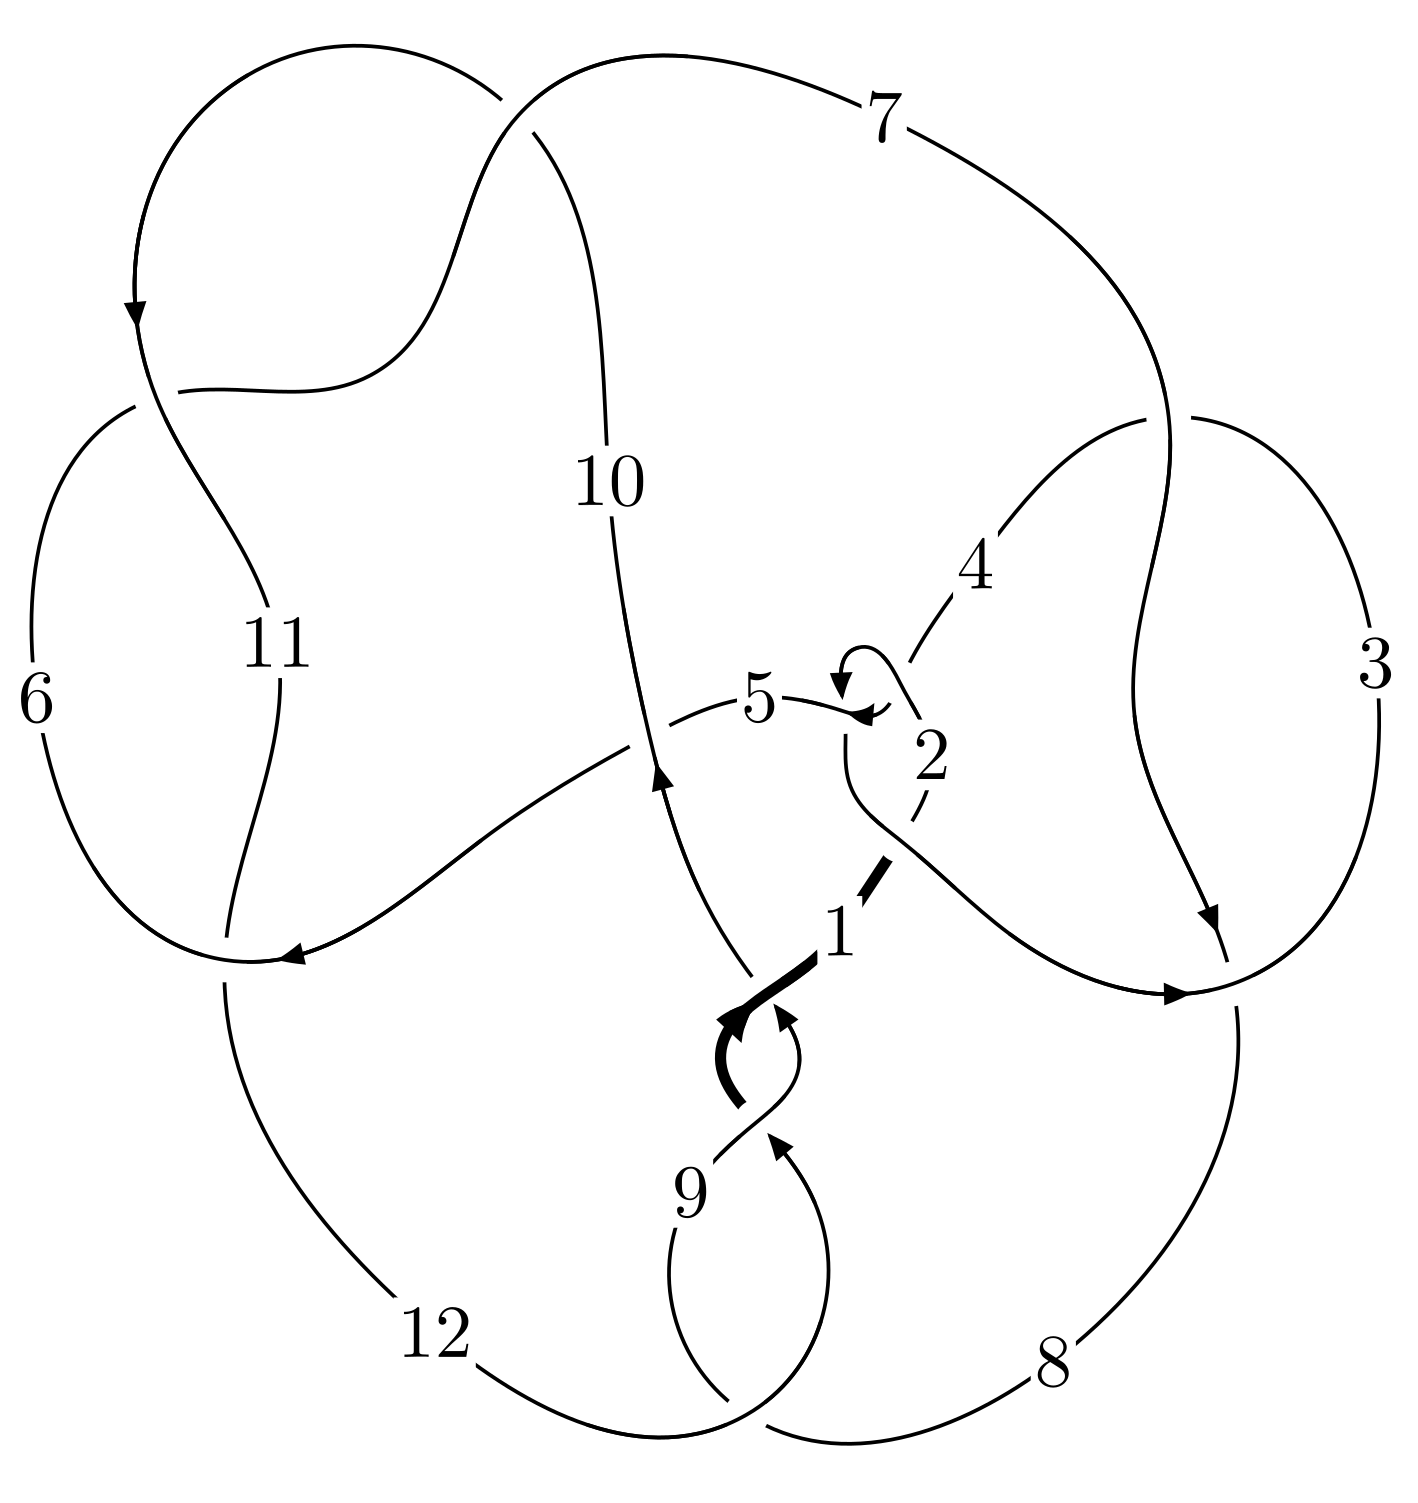
\includegraphics[width=112pt]{../../../GIT/diagram.site/Diagrams/png/2283_12n_0194.png}\\
\ \ \ A knot diagram\footnotemark}&
\allowdisplaybreaks
\textbf{Linearized knot diagam} \\
\cline{2-2}
 &
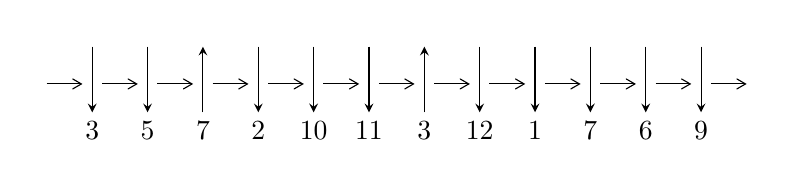
\begin{tikzpicture}[x=20pt, y=17pt]
	% nodes
	\node (C0) at (0, 0) {};
	\node (C1) at (1, 0) {};
	\node (C1U) at (1, +1) {};
	\node (C1D) at (1, -1) {3};

	\node (C2) at (2, 0) {};
	\node (C2U) at (2, +1) {};
	\node (C2D) at (2, -1) {5};

	\node (C3) at (3, 0) {};
	\node (C3U) at (3, +1) {};
	\node (C3D) at (3, -1) {7};

	\node (C4) at (4, 0) {};
	\node (C4U) at (4, +1) {};
	\node (C4D) at (4, -1) {2};

	\node (C5) at (5, 0) {};
	\node (C5U) at (5, +1) {};
	\node (C5D) at (5, -1) {10};

	\node (C6) at (6, 0) {};
	\node (C6U) at (6, +1) {};
	\node (C6D) at (6, -1) {11};

	\node (C7) at (7, 0) {};
	\node (C7U) at (7, +1) {};
	\node (C7D) at (7, -1) {3};

	\node (C8) at (8, 0) {};
	\node (C8U) at (8, +1) {};
	\node (C8D) at (8, -1) {12};

	\node (C9) at (9, 0) {};
	\node (C9U) at (9, +1) {};
	\node (C9D) at (9, -1) {1};

	\node (C10) at (10, 0) {};
	\node (C10U) at (10, +1) {};
	\node (C10D) at (10, -1) {7};

	\node (C11) at (11, 0) {};
	\node (C11U) at (11, +1) {};
	\node (C11D) at (11, -1) {6};

	\node (C12) at (12, 0) {};
	\node (C12U) at (12, +1) {};
	\node (C12D) at (12, -1) {9};
	\node (C13) at (13, 0) {};

	% arrows
	\draw[->,>={angle 60}]
	(C0) edge (C1) (C1) edge (C2) (C2) edge (C3) (C3) edge (C4) (C4) edge (C5) (C5) edge (C6) (C6) edge (C7) (C7) edge (C8) (C8) edge (C9) (C9) edge (C10) (C10) edge (C11) (C11) edge (C12) (C12) edge (C13) ;	\draw[->,>=stealth]
	(C1U) edge (C1D) (C2U) edge (C2D) (C3D) edge (C3U) (C4U) edge (C4D) (C5U) edge (C5D) (C6U) edge (C6D) (C7D) edge (C7U) (C8U) edge (C8D) (C9U) edge (C9D) (C10U) edge (C10D) (C11U) edge (C11D) (C12U) edge (C12D) ;
	\end{tikzpicture} \\
\hhline{~~} \\& 
\textbf{Solving Sequence} \\ \cline{2-2} 
 &
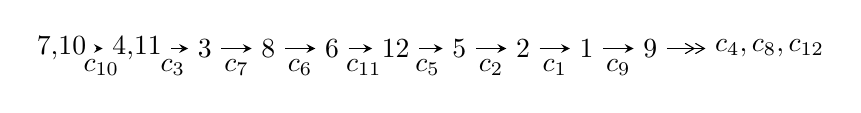
\begin{tikzpicture}[x=23pt, y=7pt]
	% node
	\node (A0) at (-1/8, 0) {7,10};
	\node (A1) at (17/16, 0) {4,11};
	\node (A2) at (17/8, 0) {3};
	\node (A3) at (25/8, 0) {8};
	\node (A4) at (33/8, 0) {6};
	\node (A5) at (41/8, 0) {12};
	\node (A6) at (49/8, 0) {5};
	\node (A7) at (57/8, 0) {2};
	\node (A8) at (65/8, 0) {1};
	\node (A9) at (73/8, 0) {9};
	\node (C1) at (1/2, -1) {$c_{10}$};
	\node (C2) at (13/8, -1) {$c_{3}$};
	\node (C3) at (21/8, -1) {$c_{7}$};
	\node (C4) at (29/8, -1) {$c_{6}$};
	\node (C5) at (37/8, -1) {$c_{11}$};
	\node (C6) at (45/8, -1) {$c_{5}$};
	\node (C7) at (53/8, -1) {$c_{2}$};
	\node (C8) at (61/8, -1) {$c_{1}$};
	\node (C9) at (69/8, -1) {$c_{9}$};
	\node (A10) at (11, 0) {$c_{4},c_{8},c_{12}$};

	% edge
	\draw[->,>=stealth]	
	(A0) edge (A1) (A1) edge (A2) (A2) edge (A3) (A3) edge (A4) (A4) edge (A5) (A5) edge (A6) (A6) edge (A7) (A7) edge (A8) (A8) edge (A9) ;
	\draw[->>,>={angle 60}]	
	(A9) edge (A10);
\end{tikzpicture} \\ 

\end{tabular} \\

\footnotetext{
The image of knot diagram is generated by the software ``\textbf{Draw programme}" developed by Andrew Bartholomew(\url{http://www.layer8.co.uk/maths/draw/index.htm\#Running-draw}), where we modified some parts for our purpose(\url{https://github.com/CATsTAILs/LinksPainter}).
}\phantom \\ \newline 
\centering \textbf{Ideals for irreducible components\footnotemark of $X_{\text{par}}$} 
 
\begin{align*}
I^u_{1}&=\langle 
1.49466\times10^{24} u^{47}-6.85289\times10^{24} u^{46}+\cdots+3.04521\times10^{25} b+1.76125\times10^{25},\\
\phantom{I^u_{1}}&\phantom{= \langle  }-7.26110\times10^{24} u^{47}-1.15653\times10^{25} u^{46}+\cdots+1.01507\times10^{25} a-1.84956\times10^{25},\;u^{48}+2 u^{47}+\cdots+2 u+1\rangle \\
I^u_{2}&=\langle 
u^5-2 u^4+5 u^3-4 u^2+3 b+3 u-1,\;a,\;u^6- u^5+3 u^4-2 u^3+2 u^2- u-1\rangle \\
\\
\end{align*}
\raggedright * 2 irreducible components of $\dim_{\mathbb{C}}=0$, with total 54 representations.\\
\footnotetext{All coefficients of polynomials are rational numbers. But the coefficients are sometimes approximated in decimal forms when there is not enough margin.}
\newpage
\renewcommand{\arraystretch}{1}
\centering \section*{I. $I^u_{1}= \langle 1.49\times10^{24} u^{47}-6.85\times10^{24} u^{46}+\cdots+3.05\times10^{25} b+1.76\times10^{25},\;-7.26\times10^{24} u^{47}-1.16\times10^{25} u^{46}+\cdots+1.02\times10^{25} a-1.85\times10^{25},\;u^{48}+2 u^{47}+\cdots+2 u+1 \rangle$}
\flushleft \textbf{(i) Arc colorings}\\
\begin{tabular}{m{7pt} m{180pt} m{7pt} m{180pt} }
\flushright $a_{7}=$&$\begin{pmatrix}0\\u\end{pmatrix}$ \\
\flushright $a_{10}=$&$\begin{pmatrix}1\\0\end{pmatrix}$ \\
\flushright $a_{4}=$&$\begin{pmatrix}0.715331 u^{47}+1.13936 u^{46}+\cdots+3.21104 u+1.82211\\-0.0490826 u^{47}+0.225039 u^{46}+\cdots-0.120857 u-0.578369\end{pmatrix}$ \\
\flushright $a_{11}=$&$\begin{pmatrix}1\\u^2\end{pmatrix}$ \\
\flushright $a_{3}=$&$\begin{pmatrix}0.715331 u^{47}+1.13936 u^{46}+\cdots+3.21104 u+1.82211\\0.101581 u^{47}+0.453744 u^{46}+\cdots-0.253590 u-0.287070\end{pmatrix}$ \\
\flushright $a_{8}=$&$\begin{pmatrix}1.02410 u^{47}+1.70903 u^{46}+\cdots-0.663879 u+2.04259\\-0.142572 u^{47}-0.142410 u^{46}+\cdots-0.481991 u-0.617041\end{pmatrix}$ \\
\flushright $a_{6}=$&$\begin{pmatrix}u\\u^3+u\end{pmatrix}$ \\
\flushright $a_{12}=$&$\begin{pmatrix}u^2+1\\u^4+2 u^2\end{pmatrix}$ \\
\flushright $a_{5}=$&$\begin{pmatrix}u^3+2 u\\u^3+u\end{pmatrix}$ \\
\flushright $a_{2}=$&$\begin{pmatrix}u^3+2 u\\-0.298901 u^{47}-0.182262 u^{46}+\cdots-0.828027 u-1.26129\end{pmatrix}$ \\
\flushright $a_{1}=$&$\begin{pmatrix}-1.47597 u^{47}-2.15015 u^{46}+\cdots+0.591045 u-4.37391\\-0.438563 u^{47}-0.494226 u^{46}+\cdots+0.0633886 u-1.37511\end{pmatrix}$ \\
\flushright $a_{9}=$&$\begin{pmatrix}1.86762 u^{47}+3.01187 u^{46}+\cdots-0.400029 u+3.80060\\0.297398 u^{47}+0.622443 u^{46}+\cdots-0.229865 u+0.150066\end{pmatrix}$\\&\end{tabular}
\flushleft \textbf{(ii) Obstruction class $= -1$}\\~\\
\flushleft \textbf{(iii) Cusp Shapes $= \frac{24180032660295489705345802}{30452057674032287811487569} u^{47}+\frac{40784802453743783652603914}{30452057674032287811487569} u^{46}+\cdots+\frac{461511678046237890102384932}{30452057674032287811487569} u-\frac{260983278311950731604691300}{30452057674032287811487569}$}\\~\\
\newpage\renewcommand{\arraystretch}{1}
\flushleft \textbf{(iv) u-Polynomials at the component}\newline \\
\begin{tabular}{m{50pt}|m{274pt}}
Crossings & \hspace{64pt}u-Polynomials at each crossing \\
\hline $$\begin{aligned}c_{1}\end{aligned}$$&$\begin{aligned}
&u^{48}+17 u^{47}+\cdots+7933 u+81
\end{aligned}$\\
\hline $$\begin{aligned}c_{2},c_{4}\end{aligned}$$&$\begin{aligned}
&u^{48}-7 u^{47}+\cdots-133 u+9
\end{aligned}$\\
\hline $$\begin{aligned}c_{3},c_{7}\end{aligned}$$&$\begin{aligned}
&u^{48}-3 u^{47}+\cdots-1344 u+576
\end{aligned}$\\
\hline $$\begin{aligned}c_{5}\end{aligned}$$&$\begin{aligned}
&u^{48}-2 u^{47}+\cdots-4494 u+1721
\end{aligned}$\\
\hline $$\begin{aligned}c_{6},c_{10},c_{11}\end{aligned}$$&$\begin{aligned}
&u^{48}+2 u^{47}+\cdots+2 u+1
\end{aligned}$\\
\hline $$\begin{aligned}c_{8},c_{9},c_{12}\end{aligned}$$&$\begin{aligned}
&u^{48}+2 u^{47}+\cdots+2 u+1
\end{aligned}$\\
\hline
\end{tabular}\\~\\
\newpage\renewcommand{\arraystretch}{1}
\flushleft \textbf{(v) Riley Polynomials at the component}\newline \\
\begin{tabular}{m{50pt}|m{274pt}}
Crossings & \hspace{64pt}Riley Polynomials at each crossing \\
\hline $$\begin{aligned}c_{1}\end{aligned}$$&$\begin{aligned}
&y^{48}+35 y^{47}+\cdots-36429289 y+6561
\end{aligned}$\\
\hline $$\begin{aligned}c_{2},c_{4}\end{aligned}$$&$\begin{aligned}
&y^{48}-17 y^{47}+\cdots-7933 y+81
\end{aligned}$\\
\hline $$\begin{aligned}c_{3},c_{7}\end{aligned}$$&$\begin{aligned}
&y^{48}-39 y^{47}+\cdots-8331264 y+331776
\end{aligned}$\\
\hline $$\begin{aligned}c_{5}\end{aligned}$$&$\begin{aligned}
&y^{48}+22 y^{47}+\cdots+1757040 y+2961841
\end{aligned}$\\
\hline $$\begin{aligned}c_{6},c_{10},c_{11}\end{aligned}$$&$\begin{aligned}
&y^{48}+46 y^{47}+\cdots-16 y+1
\end{aligned}$\\
\hline $$\begin{aligned}c_{8},c_{9},c_{12}\end{aligned}$$&$\begin{aligned}
&y^{48}-38 y^{47}+\cdots-16 y+1
\end{aligned}$\\
\hline
\end{tabular}\\~\\
\newpage\flushleft \textbf{(vi) Complex Volumes and Cusp Shapes}
$$\begin{array}{c|c|c}  
\text{Solutions to }I^u_{1}& \I (\text{vol} + \sqrt{-1}CS) & \text{Cusp shape}\\
 \hline 
\begin{aligned}
u &= -0.690041 + 0.629311 I \\
a &= \phantom{-}1.34542 + 0.54858 I \\
b &= \phantom{-}0.393714 + 0.635247 I\end{aligned}
 & -0.39368 - 5.38356 I & -9.68744 + 3.01224 I \\ \hline\begin{aligned}
u &= -0.690041 - 0.629311 I \\
a &= \phantom{-}1.34542 - 0.54858 I \\
b &= \phantom{-}0.393714 - 0.635247 I\end{aligned}
 & -0.39368 + 5.38356 I & -9.68744 - 3.01224 I \\ \hline\begin{aligned}
u &= \phantom{-}0.920254\phantom{ +0.000000I} \\
a &= \phantom{-}0.610728\phantom{ +0.000000I} \\
b &= \phantom{-}0.171718\phantom{ +0.000000I}\end{aligned}
 & -8.80254\phantom{ +0.000000I} & -4.25000\phantom{ +0.000000I} \\ \hline\begin{aligned}
u &= -0.782668 + 0.456230 I \\
a &= -0.93137 - 1.43141 I \\
b &= \phantom{-}0.071750 - 1.022760 I\end{aligned}
 & -0.95064 + 10.34180 I & -10.86039 - 7.63801 I \\ \hline\begin{aligned}
u &= -0.782668 - 0.456230 I \\
a &= -0.93137 + 1.43141 I \\
b &= \phantom{-}0.071750 + 1.022760 I\end{aligned}
 & -0.95064 - 10.34180 I & -10.86039 + 7.63801 I \\ \hline\begin{aligned}
u &= \phantom{-}0.752519 + 0.427199 I \\
a &= \phantom{-}1.20108 - 1.15434 I \\
b &= \phantom{-}0.232758 - 0.968603 I\end{aligned}
 & \phantom{-}3.81939 - 5.33756 I & -6.88950 + 5.69391 I \\ \hline\begin{aligned}
u &= \phantom{-}0.752519 - 0.427199 I \\
a &= \phantom{-}1.20108 + 1.15434 I \\
b &= \phantom{-}0.232758 + 0.968603 I\end{aligned}
 & \phantom{-}3.81939 + 5.33756 I & -6.88950 - 5.69391 I \\ \hline\begin{aligned}
u &= \phantom{-}0.628454 + 0.590544 I \\
a &= -1.21299 + 1.06633 I \\
b &= -0.215800 + 0.693349 I\end{aligned}
 & \phantom{-}4.41535 + 0.69519 I & -5.16048 + 0.01684 I \\ \hline\begin{aligned}
u &= \phantom{-}0.628454 - 0.590544 I \\
a &= -1.21299 - 1.06633 I \\
b &= -0.215800 - 0.693349 I\end{aligned}
 & \phantom{-}4.41535 - 0.69519 I & -5.16048 - 0.01684 I \\ \hline\begin{aligned}
u &= -0.173421 + 1.158010 I \\
a &= \phantom{-}0.104728 + 0.511624 I \\
b &= \phantom{-}0.326208 + 0.117818 I\end{aligned}
 & \phantom{-}2.41934 + 2.18121 I & -2.04928 - 4.16619 I\\
 \hline 
 \end{array}$$\newpage$$\begin{array}{c|c|c}  
\text{Solutions to }I^u_{1}& \I (\text{vol} + \sqrt{-1}CS) & \text{Cusp shape}\\
 \hline 
\begin{aligned}
u &= -0.173421 - 1.158010 I \\
a &= \phantom{-}0.104728 - 0.511624 I \\
b &= \phantom{-}0.326208 - 0.117818 I\end{aligned}
 & \phantom{-}2.41934 - 2.18121 I & -2.04928 + 4.16619 I \\ \hline\begin{aligned}
u &= -0.700574 + 0.375620 I \\
a &= -1.38109 - 0.68287 I \\
b &= -0.565990 - 0.710333 I\end{aligned}
 & \phantom{-}0.679050 + 0.119673 I & -8.77552 - 2.21849 I \\ \hline\begin{aligned}
u &= -0.700574 - 0.375620 I \\
a &= -1.38109 + 0.68287 I \\
b &= -0.565990 + 0.710333 I\end{aligned}
 & \phantom{-}0.679050 - 0.119673 I & -8.77552 + 2.21849 I \\ \hline\begin{aligned}
u &= -0.582865 + 0.514097 I \\
a &= \phantom{-}0.93465 + 1.68545 I \\
b &= \phantom{-}0.017056 + 0.699009 I\end{aligned}
 & \phantom{-}1.22382 + 4.04218 I & -8.14910 - 5.14084 I \\ \hline\begin{aligned}
u &= -0.582865 - 0.514097 I \\
a &= \phantom{-}0.93465 - 1.68545 I \\
b &= \phantom{-}0.017056 - 0.699009 I\end{aligned}
 & \phantom{-}1.22382 - 4.04218 I & -8.14910 + 5.14084 I \\ \hline\begin{aligned}
u &= -0.073726 + 1.279840 I \\
a &= \phantom{-}0.763442 + 1.165900 I \\
b &= \phantom{-}0.95067 + 2.94188 I\end{aligned}
 & -2.23973 + 2.01164 I & \phantom{-0.000000 } 0 \\ \hline\begin{aligned}
u &= -0.073726 - 1.279840 I \\
a &= \phantom{-}0.763442 - 1.165900 I \\
b &= \phantom{-}0.95067 - 2.94188 I\end{aligned}
 & -2.23973 - 2.01164 I & \phantom{-0.000000 } 0 \\ \hline\begin{aligned}
u &= \phantom{-}0.454285 + 1.267740 I \\
a &= -0.084057 + 0.439948 I \\
b &= -0.212998 + 0.558035 I\end{aligned}
 & -4.87446 - 4.89245 I & \phantom{-0.000000 } 0 \\ \hline\begin{aligned}
u &= \phantom{-}0.454285 - 1.267740 I \\
a &= -0.084057 - 0.439948 I \\
b &= -0.212998 - 0.558035 I\end{aligned}
 & -4.87446 + 4.89245 I & \phantom{-0.000000 } 0 \\ \hline\begin{aligned}
u &= \phantom{-}0.039248 + 1.349580 I \\
a &= -0.345427 + 0.509536 I \\
b &= \phantom{-}0.63799 + 2.52080 I\end{aligned}
 & \phantom{-}2.14165 - 1.06169 I & \phantom{-0.000000 } 0\\
 \hline 
 \end{array}$$\newpage$$\begin{array}{c|c|c}  
\text{Solutions to }I^u_{1}& \I (\text{vol} + \sqrt{-1}CS) & \text{Cusp shape}\\
 \hline 
\begin{aligned}
u &= \phantom{-}0.039248 - 1.349580 I \\
a &= -0.345427 - 0.509536 I \\
b &= \phantom{-}0.63799 - 2.52080 I\end{aligned}
 & \phantom{-}2.14165 + 1.06169 I & \phantom{-0.000000 } 0 \\ \hline\begin{aligned}
u &= \phantom{-}0.155366 + 1.377490 I \\
a &= -1.307130 - 0.198976 I \\
b &= -2.06559 - 0.51195 I\end{aligned}
 & \phantom{-}0.76215 - 5.52514 I & \phantom{-0.000000 } 0 \\ \hline\begin{aligned}
u &= \phantom{-}0.155366 - 1.377490 I \\
a &= -1.307130 + 0.198976 I \\
b &= -2.06559 + 0.51195 I\end{aligned}
 & \phantom{-}0.76215 + 5.52514 I & \phantom{-0.000000 } 0 \\ \hline\begin{aligned}
u &= -0.116249 + 1.408890 I \\
a &= \phantom{-}0.761077 - 0.196541 I \\
b &= \phantom{-}0.629505 - 0.923500 I\end{aligned}
 & \phantom{-}4.62872 + 2.83878 I & \phantom{-0.000000 } 0 \\ \hline\begin{aligned}
u &= -0.116249 - 1.408890 I \\
a &= \phantom{-}0.761077 + 0.196541 I \\
b &= \phantom{-}0.629505 + 0.923500 I\end{aligned}
 & \phantom{-}4.62872 - 2.83878 I & \phantom{-0.000000 } 0 \\ \hline\begin{aligned}
u &= \phantom{-}0.062207 + 1.412420 I \\
a &= -0.430089 + 0.015361 I \\
b &= \phantom{-}1.62377 - 1.63866 I\end{aligned}
 & \phantom{-}2.19914 - 0.22626 I & \phantom{-0.000000 } 0 \\ \hline\begin{aligned}
u &= \phantom{-}0.062207 - 1.412420 I \\
a &= -0.430089 - 0.015361 I \\
b &= \phantom{-}1.62377 + 1.63866 I\end{aligned}
 & \phantom{-}2.19914 + 0.22626 I & \phantom{-0.000000 } 0 \\ \hline\begin{aligned}
u &= \phantom{-}0.502435 + 0.225000 I \\
a &= \phantom{-}1.62411 + 2.01656 I \\
b &= -0.083166 + 0.268273 I\end{aligned}
 & -4.30776 - 3.16023 I & -15.4533 + 7.2289 I \\ \hline\begin{aligned}
u &= \phantom{-}0.502435 - 0.225000 I \\
a &= \phantom{-}1.62411 - 2.01656 I \\
b &= -0.083166 - 0.268273 I\end{aligned}
 & -4.30776 + 3.16023 I & -15.4533 - 7.2289 I \\ \hline\begin{aligned}
u &= -0.27530 + 1.46413 I \\
a &= -0.012438 + 0.946406 I \\
b &= \phantom{-}1.06530 + 2.28274 I\end{aligned}
 & \phantom{-}6.60020 + 3.71986 I & \phantom{-0.000000 } 0\\
 \hline 
 \end{array}$$\newpage$$\begin{array}{c|c|c}  
\text{Solutions to }I^u_{1}& \I (\text{vol} + \sqrt{-1}CS) & \text{Cusp shape}\\
 \hline 
\begin{aligned}
u &= -0.27530 - 1.46413 I \\
a &= -0.012438 - 0.946406 I \\
b &= \phantom{-}1.06530 - 2.28274 I\end{aligned}
 & \phantom{-}6.60020 - 3.71986 I & \phantom{-0.000000 } 0 \\ \hline\begin{aligned}
u &= -0.497658\phantom{ +0.000000I} \\
a &= -2.81262\phantom{ +0.000000I} \\
b &= \phantom{-}0.489265\phantom{ +0.000000I}\end{aligned}
 & -5.97931\phantom{ +0.000000I} & -18.9670\phantom{ +0.000000I} \\ \hline\begin{aligned}
u &= -0.20208 + 1.49219 I \\
a &= \phantom{-}0.230181 - 1.263210 I \\
b &= \phantom{-}0.03507 - 3.40945 I\end{aligned}
 & \phantom{-}7.72797 + 6.91935 I & \phantom{-0.000000 } 0 \\ \hline\begin{aligned}
u &= -0.20208 - 1.49219 I \\
a &= \phantom{-}0.230181 + 1.263210 I \\
b &= \phantom{-}0.03507 + 3.40945 I\end{aligned}
 & \phantom{-}7.72797 - 6.91935 I & \phantom{-0.000000 } 0 \\ \hline\begin{aligned}
u &= \phantom{-}0.27968 + 1.48874 I \\
a &= \phantom{-}0.168905 + 1.066710 I \\
b &= -0.65284 + 2.93812 I\end{aligned}
 & \phantom{-}10.01550 - 9.11070 I & \phantom{-0.000000 } 0 \\ \hline\begin{aligned}
u &= \phantom{-}0.27968 - 1.48874 I \\
a &= \phantom{-}0.168905 - 1.066710 I \\
b &= -0.65284 - 2.93812 I\end{aligned}
 & \phantom{-}10.01550 + 9.11070 I & \phantom{-0.000000 } 0 \\ \hline\begin{aligned}
u &= -0.28574 + 1.50317 I \\
a &= -0.330652 + 1.097020 I \\
b &= \phantom{-}0.10316 + 3.23436 I\end{aligned}
 & \phantom{-}5.3958 + 14.2406 I & \phantom{-0.000000 } 0 \\ \hline\begin{aligned}
u &= -0.28574 - 1.50317 I \\
a &= -0.330652 - 1.097020 I \\
b &= \phantom{-}0.10316 - 3.23436 I\end{aligned}
 & \phantom{-}5.3958 - 14.2406 I & \phantom{-0.000000 } 0 \\ \hline\begin{aligned}
u &= \phantom{-}0.19752 + 1.51758 I \\
a &= \phantom{-}0.024863 - 1.091200 I \\
b &= \phantom{-}0.57543 - 3.00555 I\end{aligned}
 & \phantom{-}11.29460 - 2.26941 I & \phantom{-0.000000 } 0 \\ \hline\begin{aligned}
u &= \phantom{-}0.19752 - 1.51758 I \\
a &= \phantom{-}0.024863 + 1.091200 I \\
b &= \phantom{-}0.57543 + 3.00555 I\end{aligned}
 & \phantom{-}11.29460 + 2.26941 I & \phantom{-0.000000 } 0\\
 \hline 
 \end{array}$$\newpage$$\begin{array}{c|c|c}  
\text{Solutions to }I^u_{1}& \I (\text{vol} + \sqrt{-1}CS) & \text{Cusp shape}\\
 \hline 
\begin{aligned}
u &= -0.374037 + 0.273421 I \\
a &= -0.98022 + 1.25843 I \\
b &= \phantom{-}0.051210 + 0.628665 I\end{aligned}
 & -0.755503 + 1.062600 I & -8.41291 - 6.25143 I \\ \hline\begin{aligned}
u &= -0.374037 - 0.273421 I \\
a &= -0.98022 - 1.25843 I \\
b &= \phantom{-}0.051210 - 0.628665 I\end{aligned}
 & -0.755503 - 1.062600 I & -8.41291 + 6.25143 I \\ \hline\begin{aligned}
u &= -0.19300 + 1.54906 I \\
a &= -0.209237 - 0.861034 I \\
b &= -0.98283 - 2.41559 I\end{aligned}
 & \phantom{-}6.83914 - 2.22391 I & \phantom{-0.000000 } 0 \\ \hline\begin{aligned}
u &= -0.19300 - 1.54906 I \\
a &= -0.209237 + 0.861034 I \\
b &= -0.98283 + 2.41559 I\end{aligned}
 & \phantom{-}6.83914 + 2.22391 I & \phantom{-0.000000 } 0 \\ \hline\begin{aligned}
u &= \phantom{-}0.220939 + 0.378134 I \\
a &= \phantom{-}0.89297 + 1.37411 I \\
b &= \phantom{-}0.48463 + 1.82610 I\end{aligned}
 & -3.36304 + 0.79471 I & -10.44549 + 7.25850 I \\ \hline\begin{aligned}
u &= \phantom{-}0.220939 - 0.378134 I \\
a &= \phantom{-}0.89297 - 1.37411 I \\
b &= \phantom{-}0.48463 - 1.82610 I\end{aligned}
 & -3.36304 - 0.79471 I & -10.44549 - 7.25850 I \\ \hline\begin{aligned}
u &= -0.419380\phantom{ +0.000000I} \\
a &= -0.806662\phantom{ +0.000000I} \\
b &= -0.421185\phantom{ +0.000000I}\end{aligned}
 & -0.865778\phantom{ +0.000000I} & -11.4160\phantom{ +0.000000I} \\ \hline\begin{aligned}
u &= \phantom{-}0.310865\phantom{ +0.000000I} \\
a &= \phantom{-}1.35509\phantom{ +0.000000I} \\
b &= -1.07781\phantom{ +0.000000I}\end{aligned}
 & -2.07975\phantom{ +0.000000I} & \phantom{-}2.78660\phantom{ +0.000000I}\\
 \hline 
 \end{array}$$\newpage\newpage\renewcommand{\arraystretch}{1}
\centering \section*{II. $I^u_{2}= \langle u^5-2 u^4+5 u^3-4 u^2+3 b+3 u-1,\;a,\;u^6- u^5+3 u^4-2 u^3+2 u^2- u-1 \rangle$}
\flushleft \textbf{(i) Arc colorings}\\
\begin{tabular}{m{7pt} m{180pt} m{7pt} m{180pt} }
\flushright $a_{7}=$&$\begin{pmatrix}0\\u\end{pmatrix}$ \\
\flushright $a_{10}=$&$\begin{pmatrix}1\\0\end{pmatrix}$ \\
\flushright $a_{4}=$&$\begin{pmatrix}0\\-\frac{1}{3} u^5+\frac{2}{3} u^4+\cdots- u+\frac{1}{3}\end{pmatrix}$ \\
\flushright $a_{11}=$&$\begin{pmatrix}1\\u^2\end{pmatrix}$ \\
\flushright $a_{3}=$&$\begin{pmatrix}0\\-\frac{1}{3} u^5+\frac{2}{3} u^4+\cdots- u+\frac{1}{3}\end{pmatrix}$ \\
\flushright $a_{8}=$&$\begin{pmatrix}0\\u\end{pmatrix}$ \\
\flushright $a_{6}=$&$\begin{pmatrix}u\\u^3+u\end{pmatrix}$ \\
\flushright $a_{12}=$&$\begin{pmatrix}u^2+1\\u^4+2 u^2\end{pmatrix}$ \\
\flushright $a_{5}=$&$\begin{pmatrix}u^3+2 u\\u^3+u\end{pmatrix}$ \\
\flushright $a_{2}=$&$\begin{pmatrix}- u^3-2 u\\-\frac{1}{3} u^5+\frac{2}{3} u^4+\cdots-2 u+\frac{1}{3}\end{pmatrix}$ \\
\flushright $a_{1}=$&$\begin{pmatrix}- u^3-2 u\\- u^3- u\end{pmatrix}$ \\
\flushright $a_{9}=$&$\begin{pmatrix}- u^5-2 u^3- u\\- u^5+u^4-2 u^3+u^2- u-1\end{pmatrix}$\\&\end{tabular}
\flushleft \textbf{(ii) Obstruction class $= 1$}\\~\\
\flushleft \textbf{(iii) Cusp Shapes $= \frac{7}{9} u^5-\frac{41}{9} u^4+\frac{62}{9} u^3-\frac{103}{9} u^2+6 u-\frac{178}{9}$}\\~\\
\newpage\renewcommand{\arraystretch}{1}
\flushleft \textbf{(iv) u-Polynomials at the component}\newline \\
\begin{tabular}{m{50pt}|m{274pt}}
Crossings & \hspace{64pt}u-Polynomials at each crossing \\
\hline $$\begin{aligned}c_{1},c_{2}\end{aligned}$$&$\begin{aligned}
&(u-1)^6
\end{aligned}$\\
\hline $$\begin{aligned}c_{3},c_{7}\end{aligned}$$&$\begin{aligned}
&u^6
\end{aligned}$\\
\hline $$\begin{aligned}c_{4}\end{aligned}$$&$\begin{aligned}
&(u+1)^6
\end{aligned}$\\
\hline $$\begin{aligned}c_{5},c_{8},c_{9}\end{aligned}$$&$\begin{aligned}
&u^6- u^5-3 u^4+2 u^3+2 u^2+u-1
\end{aligned}$\\
\hline $$\begin{aligned}c_{6}\end{aligned}$$&$\begin{aligned}
&u^6+u^5+3 u^4+2 u^3+2 u^2+u-1
\end{aligned}$\\
\hline $$\begin{aligned}c_{10},c_{11}\end{aligned}$$&$\begin{aligned}
&u^6- u^5+3 u^4-2 u^3+2 u^2- u-1
\end{aligned}$\\
\hline $$\begin{aligned}c_{12}\end{aligned}$$&$\begin{aligned}
&u^6+u^5-3 u^4-2 u^3+2 u^2- u-1
\end{aligned}$\\
\hline
\end{tabular}\\~\\
\newpage\renewcommand{\arraystretch}{1}
\flushleft \textbf{(v) Riley Polynomials at the component}\newline \\
\begin{tabular}{m{50pt}|m{274pt}}
Crossings & \hspace{64pt}Riley Polynomials at each crossing \\
\hline $$\begin{aligned}c_{1},c_{2},c_{4}\end{aligned}$$&$\begin{aligned}
&(y-1)^6
\end{aligned}$\\
\hline $$\begin{aligned}c_{3},c_{7}\end{aligned}$$&$\begin{aligned}
&y^6
\end{aligned}$\\
\hline $$\begin{aligned}c_{5},c_{8},c_{9}\\c_{12}\end{aligned}$$&$\begin{aligned}
&y^6-7 y^5+17 y^4-16 y^3+6 y^2-5 y+1
\end{aligned}$\\
\hline $$\begin{aligned}c_{6},c_{10},c_{11}\end{aligned}$$&$\begin{aligned}
&y^6+5 y^5+9 y^4+4 y^3-6 y^2-5 y+1
\end{aligned}$\\
\hline
\end{tabular}\\~\\
\newpage\flushleft \textbf{(vi) Complex Volumes and Cusp Shapes}
$$\begin{array}{c|c|c}  
\text{Solutions to }I^u_{2}& \I (\text{vol} + \sqrt{-1}CS) & \text{Cusp shape}\\
 \hline 
\begin{aligned}
u &= \phantom{-}0.873214\phantom{ +0.000000I} \\
a &= \phantom{-0.000000 } 0 \\
b &= -0.414549\phantom{ +0.000000I}\end{aligned}
 & -9.30502\phantom{ +0.000000I} & -20.9320\phantom{ +0.000000I} \\ \hline\begin{aligned}
u &= -0.138835 + 1.234450 I \\
a &= \phantom{-0.000000 } 0 \\
b &= -0.632705 + 1.176960 I\end{aligned}
 & \phantom{-}1.31531 + 1.97241 I & -10.03735 - 3.88708 I \\ \hline\begin{aligned}
u &= -0.138835 - 1.234450 I \\
a &= \phantom{-0.000000 } 0 \\
b &= -0.632705 - 1.176960 I\end{aligned}
 & \phantom{-}1.31531 - 1.97241 I & -10.03735 + 3.88708 I \\ \hline\begin{aligned}
u &= \phantom{-}0.408802 + 1.276380 I \\
a &= \phantom{-0.000000 } 0 \\
b &= \phantom{-}0.449122 + 0.449614 I\end{aligned}
 & -5.34051 - 4.59213 I & -15.2999 - 0.2296 I \\ \hline\begin{aligned}
u &= \phantom{-}0.408802 - 1.276380 I \\
a &= \phantom{-0.000000 } 0 \\
b &= \phantom{-}0.449122 - 0.449614 I\end{aligned}
 & -5.34051 + 4.59213 I & -15.2999 + 0.2296 I \\ \hline\begin{aligned}
u &= -0.413150\phantom{ +0.000000I} \\
a &= \phantom{-0.000000 } 0 \\
b &= \phantom{-}1.11505\phantom{ +0.000000I}\end{aligned}
 & -2.38379\phantom{ +0.000000I} & -24.8380\phantom{ +0.000000I}\\
 \hline 
 \end{array}$$\newpage
\newpage\renewcommand{\arraystretch}{1}
\centering \section*{ III. u-Polynomials}
\begin{tabular}{m{50pt}|m{274pt}}
Crossings & \hspace{64pt}u-Polynomials at each crossing \\
\hline $$\begin{aligned}c_{1}\end{aligned}$$&$\begin{aligned}
&((u-1)^6)(u^{48}+17 u^{47}+\cdots+7933 u+81)
\end{aligned}$\\
\hline $$\begin{aligned}c_{2}\end{aligned}$$&$\begin{aligned}
&((u-1)^6)(u^{48}-7 u^{47}+\cdots-133 u+9)
\end{aligned}$\\
\hline $$\begin{aligned}c_{3},c_{7}\end{aligned}$$&$\begin{aligned}
&u^6(u^{48}-3 u^{47}+\cdots-1344 u+576)
\end{aligned}$\\
\hline $$\begin{aligned}c_{4}\end{aligned}$$&$\begin{aligned}
&((u+1)^6)(u^{48}-7 u^{47}+\cdots-133 u+9)
\end{aligned}$\\
\hline $$\begin{aligned}c_{5}\end{aligned}$$&$\begin{aligned}
&(u^6- u^5-3 u^4+2 u^3+2 u^2+u-1)(u^{48}-2 u^{47}+\cdots-4494 u+1721)
\end{aligned}$\\
\hline $$\begin{aligned}c_{6}\end{aligned}$$&$\begin{aligned}
&(u^6+u^5+3 u^4+2 u^3+2 u^2+u-1)(u^{48}+2 u^{47}+\cdots+2 u+1)
\end{aligned}$\\
\hline $$\begin{aligned}c_{8},c_{9}\end{aligned}$$&$\begin{aligned}
&(u^6- u^5-3 u^4+2 u^3+2 u^2+u-1)(u^{48}+2 u^{47}+\cdots+2 u+1)
\end{aligned}$\\
\hline $$\begin{aligned}c_{10},c_{11}\end{aligned}$$&$\begin{aligned}
&(u^6- u^5+3 u^4-2 u^3+2 u^2- u-1)(u^{48}+2 u^{47}+\cdots+2 u+1)
\end{aligned}$\\
\hline $$\begin{aligned}c_{12}\end{aligned}$$&$\begin{aligned}
&(u^6+u^5-3 u^4-2 u^3+2 u^2- u-1)(u^{48}+2 u^{47}+\cdots+2 u+1)
\end{aligned}$\\
\hline
\end{tabular}\newpage\renewcommand{\arraystretch}{1}
\centering \section*{ IV. Riley Polynomials}
\begin{tabular}{m{50pt}|m{274pt}}
Crossings & \hspace{64pt}Riley Polynomials at each crossing \\
\hline $$\begin{aligned}c_{1}\end{aligned}$$&$\begin{aligned}
&((y-1)^6)(y^{48}+35 y^{47}+\cdots-36429289 y+6561)
\end{aligned}$\\
\hline $$\begin{aligned}c_{2},c_{4}\end{aligned}$$&$\begin{aligned}
&((y-1)^6)(y^{48}-17 y^{47}+\cdots-7933 y+81)
\end{aligned}$\\
\hline $$\begin{aligned}c_{3},c_{7}\end{aligned}$$&$\begin{aligned}
&y^6(y^{48}-39 y^{47}+\cdots-8331264 y+331776)
\end{aligned}$\\
\hline $$\begin{aligned}c_{5}\end{aligned}$$&$\begin{aligned}
&(y^6-7 y^5+17 y^4-16 y^3+6 y^2-5 y+1)\\
&\cdot(y^{48}+22 y^{47}+\cdots+1757040 y+2961841)
\end{aligned}$\\
\hline $$\begin{aligned}c_{6},c_{10},c_{11}\end{aligned}$$&$\begin{aligned}
&(y^6+5 y^5+\cdots-5 y+1)(y^{48}+46 y^{47}+\cdots-16 y+1)
\end{aligned}$\\
\hline $$\begin{aligned}c_{8},c_{9},c_{12}\end{aligned}$$&$\begin{aligned}
&(y^6-7 y^5+\cdots-5 y+1)(y^{48}-38 y^{47}+\cdots-16 y+1)
\end{aligned}$\\
\hline
\end{tabular}
\vskip 2pc
\end{document}